
\documentclass{standalone}

%\documentclass[convert]{standalone}
% convert: in addition to pdf output files, png files are created
% convert options does work properly with -output-directory option of latexmk

\usepackage{tikz-feynman}
\tikzfeynmanset{compat=1.1.0}


\begin{document}
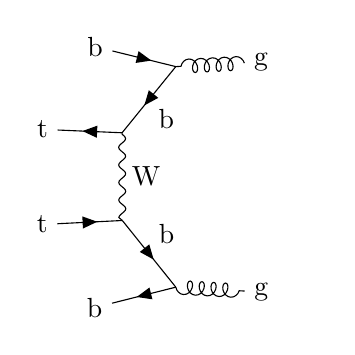
\begin{tikzpicture}
          \begin{feynman}
            \diagram [small, vertical'=a to d] {
            % t-channel ttbar, qq -> gg -- > bbtt

            gi1 [particle=g] -- [gluon] a -- [fermion, edge label=b] b -- [boson, edge label=W] c -- [fermion, edge label=b] d -- [gluon] gi2 [particle=g],

            b1 [particle=b] -- [fermion] a,
            b -- [fermion] t2 [particle=t],

            t1 [particle=t] -- [fermion] c,
            d -- [fermion] b2 [particle=b],

            % invisible helper
            gi1 -- [draw=none] inv1 -- [draw=none] inv2 -- [draw=none] gi2,
            t1 -- [draw=none] b2,
            b1 -- [draw=none] t2,
            t2 -- [draw=none] t1,
            };
          \end{feynman}
        \end{tikzpicture}
\end{document}
